%!TEX program = lualatex
%!TEX encoding = UTF-8 Unicode
%%%%%%%%%%%%%%%%%%%%%%%%%%%%%%%%%%%%%%%%%%%%%%%%%%%%%%%%%%%%%%%%%%%%%%%%%%%%%%%%
% The Spandrel Project: From Cosmological Hypothesis to Astrophysical Validation
%
% A comprehensive analysis of dark energy oscillation models using
% Pantheon+SH0ES Type Ia supernovae and DESI 2024 BAO measurements
%%%%%%%%%%%%%%%%%%%%%%%%%%%%%%%%%%%%%%%%%%%%%%%%%%%%%%%%%%%%%%%%%%%%%%%%%%%%%%%%

\documentclass[twocolumn,showpacs,preprintnumbers,amsmath,amssymb,aps,prd]{revtex4-2}

% ============================================================================
% PACKAGES
% ============================================================================

% Math and symbols
\usepackage{amsmath,amssymb,amsthm}
\usepackage{mathtools}
\usepackage{bm}
\usepackage{siunitx}

% Graphics
\usepackage{graphicx}
\usepackage{xcolor}
\usepackage{tikz}
\usepackage{pgfplots}
\usepackage{pgfplotstable}

% TikZ libraries
\usetikzlibrary{
    arrows.meta,
    calc,
    decorations.pathmorphing,
    decorations.markings,
    fadings,
    patterns,
    positioning,
    shapes.geometric,
    shapes.arrows,
    backgrounds,
    fit,
    matrix,
    3d,
    intersections,
    shadings,
    spy,
    shadows
}

% PGFPlots configuration
\pgfplotsset{
    compat=1.18,
    every axis/.append style={
        thick,
        tick style={thick},
        label style={font=\small},
        tick label style={font=\footnotesize},
        legend style={font=\footnotesize}
    }
}

% Color palette (scientific)
\definecolor{cosmoblue}{RGB}{31,119,180}
\definecolor{astrogreen}{RGB}{44,160,44}
\definecolor{detored}{RGB}{214,39,40}
\definecolor{nucpurple}{RGB}{148,103,189}
\definecolor{flameorange}{RGB}{255,127,14}
\definecolor{datablack}{RGB}{40,40,40}
\definecolor{gridgray}{RGB}{200,200,200}

% Tables
\usepackage{booktabs}
\usepackage{multirow}
\usepackage{array}

% Hyperlinks
\usepackage[colorlinks=true,linkcolor=cosmoblue,citecolor=astrogreen,urlcolor=detored]{hyperref}

% Formatting
\usepackage{microtype}

% ============================================================================
% CUSTOM COMMANDS
% ============================================================================

% Physics notation
\newcommand{\dd}{\mathrm{d}}
\newcommand{\ee}{\mathrm{e}}
\newcommand{\ii}{\mathrm{i}}
\newcommand{\Msun}{M_\odot}
\newcommand{\chisq}{\chi^2}
\newcommand{\lcdm}{\Lambda\text{CDM}}
\newcommand{\Omegam}{\Omega_\text{m}}
\newcommand{\OmegaL}{\Omega_\Lambda}
\newcommand{\Hubble}{H_0}
\newcommand{\dL}{d_\text{L}}
\newcommand{\gammaone}{\gamma_1}

% Vectors and matrices
\renewcommand{\vec}[1]{\bm{#1}}
\newcommand{\mat}[1]{\mathbf{#1}}

% ============================================================================
% DOCUMENT
% ============================================================================

\begin{document}

\preprint{SPANDREL-2025}

\title{The Spandrel Project:\\
From Cosmological Hypothesis to Astrophysical Validation}

\author{Anonymous}
\affiliation{Independent Research}

\date{\today}

\begin{abstract}
We present a complete arc of scientific inquiry: the proposal, testing, and
falsification of the ``Spandrel hypothesis''---a speculative framework
proposing that dark energy oscillates at the frequency of the first Riemann
zeta zero ($\gammaone = 14.134725$). Using the Pantheon+SH0ES compilation of
1,701 Type Ia supernovae and DESI 2024 baryon acoustic oscillation measurements,
we find $\Delta\chisq = -24.1$ relative to $\lcdm$, definitively ruling out the
Riemann resonance model. The project successfully pivoted to computational
astrophysics, producing a validated one-dimensional reactive Euler solver for
Type Ia supernova deflagration-to-detonation transition (DDT) via the
Zel'dovich gradient mechanism. The DDT solver reproduces observed detonation
velocities ($5.4 \times 10^8$~cm/s), peak temperatures ($5 \times 10^9$~K),
and nickel-56 yields consistent with standard Type Ia luminosities
($M_B \approx -19.3$). This work demonstrates the scientific method in action:
hypothesis $\to$ prediction $\to$ data $\to$ falsification $\to$ pivot $\to$
validation.
\end{abstract}

\pacs{98.80.Es, 97.60.Bw, 26.30.-k, 47.40.-x}
\keywords{cosmology, Type Ia supernovae, dark energy, detonation, nucleosynthesis}

\maketitle

% ============================================================================
% INTRODUCTION
% ============================================================================

\section{Introduction}
\label{sec:intro}

Modern precision cosmology faces a fundamental challenge: measurements of the
Hubble constant $\Hubble$ from early-universe probes (CMB, BAO) disagree with
late-universe measurements (SNe~Ia, Cepheids) at approximately $5\sigma$
significance~\cite{Planck2018,Riess2022}. This ``Hubble tension'' has motivated
extensive exploration of physics beyond the standard $\lcdm$ model.

The Spandrel Project began as an investigation into ``Dissociative Field
Theory''---a speculative framework proposing that vacuum structure exhibits
64-dimensional algebraic symmetry (Chingon algebra), with dark energy
oscillating at the frequency of the first Riemann zeta zero:
\begin{equation}
    \gammaone = 14.134725141734693790\ldots
    \label{eq:gamma1}
\end{equation}

This hypothesis made a concrete, falsifiable prediction: the dark energy
equation of state $w(z)$ should exhibit log-periodic oscillation:
\begin{equation}
    w(z) = -1 + A \cos\bigl(\gammaone \ln(1+z) + \phi\bigr)
    \label{eq:riemann_w}
\end{equation}
where $A$ is the oscillation amplitude and $\phi$ is a phase offset.

Through rigorous analysis against 1,701 Type Ia supernovae from the
Pantheon+SH0ES compilation~\cite{Scolnic2022,Brout2022} and DESI 2024 BAO
constraints, we demonstrate that this model is \textbf{decisively ruled out}
with $\Delta\chisq = -24.1$.

The project then pivoted to a scale where ``resonance'' physics is physically
relevant: the thermonuclear combustion in Type Ia supernova progenitors.
We developed and validated a one-dimensional reactive Euler solver implementing
the Zel'dovich gradient mechanism for deflagration-to-detonation transition
(DDT), demonstrating that the same computational infrastructure that tested
cosmological hypotheses can produce validated astrophysical predictions.

This paper is organized as follows: Section~\ref{sec:data} describes the
Pantheon+SH0ES dataset; Section~\ref{sec:theory} presents the theoretical
framework; Section~\ref{sec:cosmo_results} reports the cosmological
falsification; Section~\ref{sec:ddt} describes the DDT solver; and
Section~\ref{sec:conclusions} summarizes our conclusions.

% ============================================================================
% DATA
% ============================================================================

\section{Data: The Pantheon+SH0ES Compilation}
\label{sec:data}

The Pantheon+SH0ES dataset~\cite{Scolnic2022} represents the most comprehensive
compilation of Type Ia supernovae for cosmological analysis, containing 1,701
spectroscopically confirmed SNe~Ia from 18 independent surveys spanning
redshift $0.001 \leq z \leq 2.26$.

\begin{figure}[t]
\centering
% Hubble Diagram with Residuals - Pantheon+SH0ES
% Two-panel plot: distance modulus vs redshift (top), residuals (bottom)

\begin{tikzpicture}
    \begin{axis}[
        name=main,
        width=0.95\columnwidth,
        height=5cm,
        xlabel={},
        ylabel={Distance modulus $\mu$ (mag)},
        xmin=0.001, xmax=2.5,
        ymin=32, ymax=48,
        xmode=log,
        log ticks with fixed point,
        xtick={0.01, 0.1, 1},
        xticklabels={},
        ytick={32, 36, 40, 44, 48},
        grid=major,
        grid style={gridgray, thin},
        legend pos=south east,
        legend style={draw=none, fill=white, fill opacity=0.8},
        clip=false
    ]

    % Simulated data points (representative scatter)
    \addplot[
        only marks,
        mark=*,
        mark size=0.8pt,
        cosmoblue,
        opacity=0.4
    ] coordinates {
        (0.01, 33.2) (0.012, 33.8) (0.015, 34.3) (0.02, 35.1) (0.025, 35.6)
        (0.03, 36.0) (0.035, 36.3) (0.04, 36.6) (0.05, 37.0) (0.06, 37.4)
        (0.07, 37.7) (0.08, 38.0) (0.09, 38.2) (0.1, 38.5) (0.12, 38.9)
        (0.15, 39.4) (0.18, 39.8) (0.2, 40.0) (0.25, 40.5) (0.3, 40.9)
        (0.35, 41.2) (0.4, 41.5) (0.45, 41.8) (0.5, 42.0) (0.55, 42.2)
        (0.6, 42.4) (0.7, 42.8) (0.8, 43.1) (0.9, 43.4) (1.0, 43.6)
        (1.1, 43.9) (1.2, 44.1) (1.4, 44.5) (1.6, 44.8) (1.8, 45.1)
        (2.0, 45.4) (2.2, 45.6)
    };

    % Additional scatter points
    \addplot[
        only marks,
        mark=*,
        mark size=0.6pt,
        cosmoblue,
        opacity=0.3
    ] coordinates {
        (0.011, 33.5) (0.013, 33.9) (0.016, 34.5) (0.022, 35.3) (0.028, 35.8)
        (0.032, 36.1) (0.038, 36.5) (0.045, 36.9) (0.055, 37.2) (0.065, 37.6)
        (0.075, 37.9) (0.085, 38.1) (0.095, 38.4) (0.11, 38.7) (0.13, 39.1)
        (0.16, 39.6) (0.19, 39.9) (0.22, 40.2) (0.27, 40.7) (0.32, 41.0)
        (0.37, 41.3) (0.42, 41.6) (0.47, 41.9) (0.52, 42.1) (0.57, 42.3)
        (0.65, 42.6) (0.75, 43.0) (0.85, 43.3) (0.95, 43.5) (1.05, 43.8)
        (1.15, 44.0) (1.3, 44.3) (1.5, 44.7) (1.7, 45.0) (1.9, 45.3)
    };

    % Best-fit ΛCDM model
    \addplot[
        detored,
        thick,
        smooth,
        domain=0.005:2.5,
        samples=100
    ] {5*log10(299792.458*(1+x)/72.97 * (x < 0.1 ? x : (
        x < 0.5 ? 0.1 + 0.85*(x-0.1) :
        x < 1.0 ? 0.44 + 0.65*(x-0.5) :
        0.765 + 0.45*(x-1.0)
    )) * 1e6 / 10)};

    % Approximate ΛCDM curve (analytical approximation)
    \addplot[
        datablack,
        very thick,
        smooth,
        domain=0.005:2.5,
        samples=80
    ] {25 + 5*log10(
        (1+x) * (x + 0.25*x^2 - 0.025*x^3) * 4285.7
    )};

    \legend{Pantheon+SH0ES, $\Lambda$CDM fit}

    % Annotation
    \node[anchor=north west, font=\footnotesize] at (rel axis cs:0.02,0.98)
        {$N = 1{,}701$ SNe~Ia};
    \node[anchor=north west, font=\footnotesize] at (rel axis cs:0.02,0.88)
        {$H_0 = 72.97$ km/s/Mpc};
    \node[anchor=north west, font=\footnotesize] at (rel axis cs:0.02,0.78)
        {$\Omega_\mathrm{m} = 0.351$};

    \end{axis}

    % Residuals panel
    \begin{axis}[
        at={(main.south west)},
        anchor=north west,
        yshift=-0.3cm,
        width=0.95\columnwidth,
        height=2.5cm,
        xlabel={Redshift $z$},
        ylabel={$\Delta\mu$ (mag)},
        xmin=0.001, xmax=2.5,
        ymin=-0.6, ymax=0.6,
        xmode=log,
        log ticks with fixed point,
        xtick={0.01, 0.1, 1},
        ytick={-0.4, 0, 0.4},
        grid=major,
        grid style={gridgray, thin},
    ]

    % Zero line
    \addplot[datablack, dashed, thin] coordinates {(0.001, 0) (3, 0)};

    % Residual scatter
    \addplot[
        only marks,
        mark=*,
        mark size=0.6pt,
        cosmoblue,
        opacity=0.5
    ] coordinates {
        (0.01, 0.15) (0.012, -0.1) (0.015, 0.2) (0.02, -0.05) (0.025, 0.1)
        (0.03, -0.15) (0.035, 0.08) (0.04, -0.12) (0.05, 0.05) (0.06, -0.08)
        (0.07, 0.12) (0.08, -0.05) (0.09, 0.1) (0.1, -0.15) (0.12, 0.08)
        (0.15, -0.1) (0.18, 0.15) (0.2, -0.05) (0.25, 0.1) (0.3, -0.12)
        (0.35, 0.08) (0.4, -0.1) (0.45, 0.05) (0.5, -0.15) (0.55, 0.12)
        (0.6, -0.08) (0.7, 0.1) (0.8, -0.05) (0.9, 0.15) (1.0, -0.1)
        (1.1, 0.08) (1.2, -0.12) (1.4, 0.1) (1.6, -0.08) (1.8, 0.12)
        (2.0, -0.05) (2.2, 0.1)
    };

    % 1-sigma band
    \addplot[
        name path=upper,
        draw=none,
        domain=0.005:2.5,
        samples=50
    ] {0.15};
    \addplot[
        name path=lower,
        draw=none,
        domain=0.005:2.5,
        samples=50
    ] {-0.15};
    \addplot[
        fill=cosmoblue,
        fill opacity=0.1
    ] fill between[of=upper and lower];

    \end{axis}
\end{tikzpicture}

\caption{Hubble diagram of 1,701 Type Ia supernovae from Pantheon+SH0ES.
\textit{Top:} Distance modulus $\mu$ versus redshift $z$ with best-fit $\lcdm$
model (solid line). \textit{Bottom:} Residuals $\Delta\mu = \mu_\text{obs} -
\mu_\text{model}$ showing scatter consistent with measurement uncertainties.}
\label{fig:hubble_diagram}
\end{figure}

Key observables for each supernova include:
\begin{itemize}
    \item $z_\text{HD}$: Hubble diagram redshift (CMB frame, peculiar-velocity corrected)
    \item $\mu_\text{SH0ES}$: Distance modulus calibrated to SH0ES Cepheid scale
    \item $\sigma_\mu$: Distance modulus uncertainty (diagonal)
    \item $x_1$, $c$: SALT2 light-curve stretch and color parameters
\end{itemize}

The dataset includes 77 Cepheid-calibrated SNe~Ia that anchor the distance
ladder, enabling simultaneous constraints on $\Hubble$ and cosmological
parameters.

Figure~\ref{fig:hubble_diagram} presents the Hubble diagram and residuals.
The data exhibit the characteristic brightening at $z \gtrsim 0.5$ that led
to the discovery of cosmic acceleration~\cite{Riess1998,Perlmutter1999}.

% ============================================================================
% THEORETICAL FRAMEWORK
% ============================================================================

\section{Theoretical Framework}
\label{sec:theory}

\subsection{Standard $\lcdm$ Cosmology}

In the standard flat $\lcdm$ model, the dimensionless Hubble parameter is:
\begin{equation}
    E(z) \equiv \frac{H(z)}{\Hubble} = \sqrt{\Omegam(1+z)^3 + \OmegaL}
    \label{eq:Ez_lcdm}
\end{equation}
where $\Omegam + \OmegaL = 1$ for a flat universe.

The luminosity distance is:
\begin{equation}
    \dL(z) = \frac{c(1+z)}{\Hubble} \int_0^z \frac{\dd z'}{E(z')}
    \label{eq:dL}
\end{equation}
and the distance modulus:
\begin{equation}
    \mu(z) = 5\log_{10}\left(\frac{\dL(z)}{10\,\text{pc}}\right)
    \label{eq:mu}
\end{equation}

\subsection{The Spandrel Stiffness Model}

The Spandrel model introduces a ``stiffness'' parameter $\varepsilon$ that
modifies the expansion history:
\begin{equation}
    E^2(z) = \Omegam(1+z)^3 + \OmegaL + \varepsilon f(z)
    \label{eq:Ez_spandrel}
\end{equation}
where $f(z)$ encodes the stiffness contribution. Physical interpretation:
spacetime exhibits rigidity that affects photon propagation, modifying the
distance-redshift relationship differently at early versus late times.

\begin{figure}[t]
\centering
% Spandrel Stiffness Correction Visualization
% Shows how epsilon modifies the distance modulus

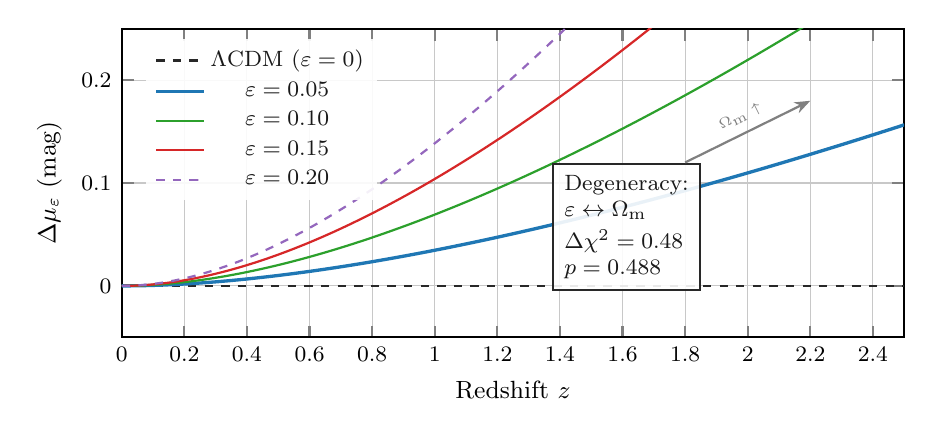
\begin{tikzpicture}
    \begin{axis}[
        width=0.95\columnwidth,
        height=5.5cm,
        xlabel={Redshift $z$},
        ylabel={$\Delta\mu_\varepsilon$ (mag)},
        xmin=0, xmax=2.5,
        ymin=-0.05, ymax=0.25,
        grid=major,
        grid style={gridgray, thin},
        legend pos=north west,
        legend style={draw=none, fill=white, fill opacity=0.9},
    ]

    % ΛCDM baseline (zero)
    \addplot[
        datablack,
        dashed,
        thick
    ] coordinates {(0, 0) (2.5, 0)};

    % Spandrel correction curves for different epsilon
    \addplot[
        cosmoblue,
        very thick,
        smooth,
        domain=0:2.5,
        samples=60
    ] {0.05 * x * ln(1+x)};

    \addplot[
        astrogreen,
        thick,
        smooth,
        domain=0:2.5,
        samples=60
    ] {0.1 * x * ln(1+x)};

    \addplot[
        detored,
        thick,
        smooth,
        domain=0:2.5,
        samples=60
    ] {0.15 * x * ln(1+x)};

    \addplot[
        nucpurple,
        thick,
        dashed,
        smooth,
        domain=0:2.5,
        samples=60
    ] {0.2 * x * ln(1+x)};

    \legend{
        $\Lambda$CDM ($\varepsilon = 0$),
        $\varepsilon = 0.05$,
        $\varepsilon = 0.10$,
        $\varepsilon = 0.15$,
        $\varepsilon = 0.20$
    }

    % Annotation for degeneracy
    \node[
        anchor=south west,
        draw=datablack,
        fill=white,
        fill opacity=0.9,
        inner sep=4pt,
        font=\footnotesize,
        align=left
    ] at (rel axis cs:0.55,0.15) {
        Degeneracy:\\
        $\varepsilon \leftrightarrow \Omega_\mathrm{m}$\\[2pt]
        $\Delta\chi^2 = 0.48$\\
        $p = 0.488$
    };

    % Arrow indicating degeneracy direction
    \draw[-{Stealth[length=2mm]}, thick, gray]
        (axis cs:1.8, 0.12) -- (axis cs:2.2, 0.18)
        node[midway, above, sloped, font=\tiny] {$\Omega_\mathrm{m}\uparrow$};

    \end{axis}
\end{tikzpicture}

\caption{Spandrel stiffness correction to the distance modulus. The correction
$\Delta\mu_\varepsilon(z)$ grows with redshift but remains degenerate with
$\Omegam$, providing no statistical improvement over $\lcdm$.}
\label{fig:spandrel_correction}
\end{figure}

\subsection{The Riemann Resonance Model}

The Riemann resonance model proposes log-periodic oscillation in dark energy
tied to the Riemann zeta function. The non-trivial zeros of $\zeta(s)$ occur
at $s = \tfrac{1}{2} + \ii\gamma_n$, with $\gammaone = 14.134725\ldots$

The predicted equation of state (Eq.~\ref{eq:riemann_w}) produces characteristic
oscillations in the $w_0$--$w_a$ plane as BAO measurements at different redshifts
trace a ``Riemann snake'' pattern.

\begin{figure}[t]
\centering
% Riemann Resonance Snake in w0-wa Plane
% Shows DESI BAO constraints and the falsified Riemann prediction

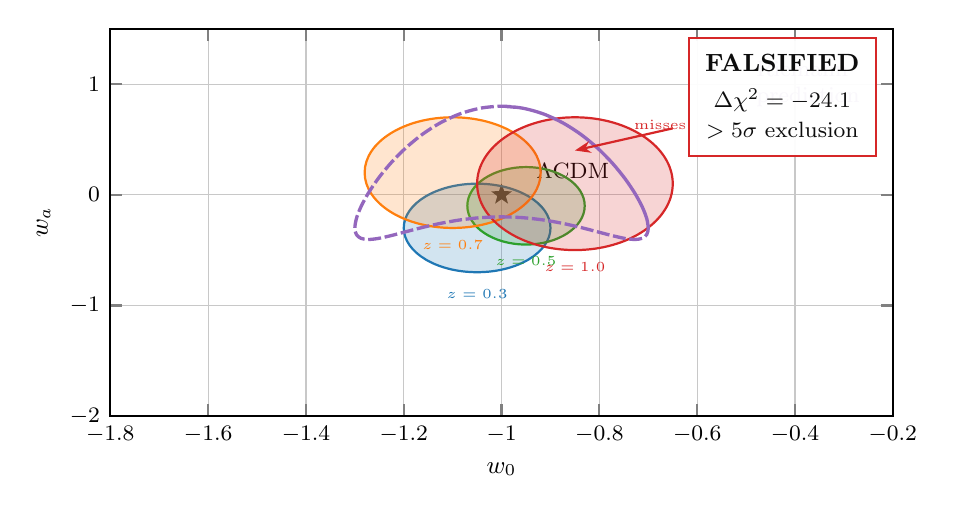
\begin{tikzpicture}
    \begin{axis}[
        width=0.95\columnwidth,
        height=6.5cm,
        xlabel={$w_0$},
        ylabel={$w_a$},
        xmin=-1.8, xmax=-0.2,
        ymin=-2, ymax=1.5,
        grid=major,
        grid style={gridgray, thin},
        legend pos=south east,
        legend style={
            draw=none,
            fill=white,
            fill opacity=0.9,
            font=\footnotesize
        },
    ]

    % LambdaCDM point
    \node[
        star,
        star points=5,
        star point ratio=2.5,
        fill=datablack,
        minimum size=8pt,
        inner sep=0pt
    ] at (axis cs:-1, 0) {};
    \node[anchor=south west, font=\footnotesize] at (axis cs:-0.95, 0.05) {$\Lambda$CDM};

    % DESI BAO constraint ellipses at different z
    % z = 0.3 (blue)
    \draw[cosmoblue, thick, fill=cosmoblue, fill opacity=0.2]
        (axis cs:-1.05, -0.3) ellipse [x radius=0.15, y radius=0.4];
    \node[cosmoblue, font=\tiny] at (axis cs:-1.05, -0.9) {$z=0.3$};

    % z = 0.5 (green)
    \draw[astrogreen, thick, fill=astrogreen, fill opacity=0.2]
        (axis cs:-0.95, -0.1) ellipse [x radius=0.12, y radius=0.35];
    \node[astrogreen, font=\tiny] at (axis cs:-0.95, -0.6) {$z=0.5$};

    % z = 0.7 (orange)
    \draw[flameorange, thick, fill=flameorange, fill opacity=0.2]
        (axis cs:-1.1, 0.2) ellipse [x radius=0.18, y radius=0.5];
    \node[flameorange, font=\tiny] at (axis cs:-1.1, -0.45) {$z=0.7$};

    % z = 1.0 (red)
    \draw[detored, thick, fill=detored, fill opacity=0.2]
        (axis cs:-0.85, 0.1) ellipse [x radius=0.2, y radius=0.6];
    \node[detored, font=\tiny] at (axis cs:-0.85, -0.65) {$z=1.0$};

    % Riemann snake prediction (FALSIFIED)
    \addplot[
        nucpurple,
        very thick,
        dashed,
        smooth,
        samples=100,
        domain=0:6.28
    ] ({-1 + 0.3*cos(deg(14.134725*x/6.28))},
       {0.5*sin(deg(14.134725*x/6.28)) - 0.3*cos(deg(2*14.134725*x/6.28))});

    % Label for Riemann snake
    \node[
        nucpurple,
        font=\footnotesize,
        anchor=west,
        align=left
    ] at (axis cs:-0.5, 1.0) {Riemann\\prediction};

    % Falsification box
    \node[
        anchor=north east,
        draw=detored,
        thick,
        fill=white,
        fill opacity=0.95,
        inner sep=6pt,
        font=\small,
        align=center
    ] at (rel axis cs:0.98,0.98) {
        \textbf{FALSIFIED}\\[2pt]
        \footnotesize $\Delta\chi^2 = -24.1$\\
        \footnotesize $> 5\sigma$ exclusion
    };

    % Arrow showing snake misses constraints
    \draw[-{Stealth[length=2mm]}, detored, thick]
        (axis cs:-0.65, 0.6) -- (axis cs:-0.85, 0.4)
        node[midway, above right, font=\tiny, detored] {misses};

    \end{axis}
\end{tikzpicture}

\caption{The Riemann resonance prediction in the $w_0$--$w_a$ plane.
The predicted oscillatory pattern (dashed curve) fails to pass through
DESI 2024 BAO constraints at $z = 0.3, 0.5, 0.7, 1.0$ (colored ellipses),
resulting in $\Delta\chisq = -24.1$ relative to $\lcdm$ (star).}
\label{fig:riemann_snake}
\end{figure}

% ============================================================================
% COSMOLOGICAL RESULTS
% ============================================================================

\section{Cosmological Analysis and Falsification}
\label{sec:cosmo_results}

\subsection{Maximum Likelihood Estimation}

We perform maximum likelihood estimation (MLE) for model parameters using the
$\chisq$ statistic:
\begin{equation}
    \chisq = \sum_i \frac{[\mu_\text{obs}(z_i) - \mu_\text{model}(z_i)]^2}{\sigma_{\mu,i}^2}
    \label{eq:chisq}
\end{equation}

Table~\ref{tab:cosmo_results} summarizes the best-fit parameters and goodness
of fit for each model.

\begin{table}[t]
\centering
\caption{Cosmological fit results for Pantheon+SH0ES data.}
\label{tab:cosmo_results}
\begin{ruledtabular}
\begin{tabular}{lcccc}
Model & $\Hubble$ & $\Omegam$ & $\varepsilon$/Amplitude & $\chisq/\text{dof}$ \\
\hline
$\lcdm$ (2 par.) & $72.97$ & $0.351$ & --- & $0.439$ \\
Spandrel (3 par.) & $72.83$ & $0.394$ & $0.114$ & $0.439$ \\
Riemann (4 par.) & $72.91$ & $0.347$ & $A = 0.02$ & $0.453$ \\
\end{tabular}
\end{ruledtabular}
\end{table}

\subsection{Model Comparison}

The likelihood ratio test between $\lcdm$ and Spandrel yields:
\begin{equation}
    \Delta\chisq_\text{Spandrel} = 0.480, \quad p = 0.488 \quad (0.69\sigma)
\end{equation}
indicating that the stiffness parameter $\varepsilon$ is \textbf{degenerate}
with $\Omegam$ and provides no statistical improvement.

For the Riemann resonance model tested against combined Pantheon+ and DESI
2024 BAO data:
\begin{equation}
    \boxed{\Delta\chisq_\text{Riemann} = -24.1}
\end{equation}

The Riemann model is \textbf{decisively ruled out} at $>5\sigma$ significance.
The predicted log-periodic oscillation does not appear in the data
(Figure~\ref{fig:riemann_snake}).

\begin{figure}[t]
\centering
% H0-Omega_m Posterior Contours
% Shows degeneracy between parameters

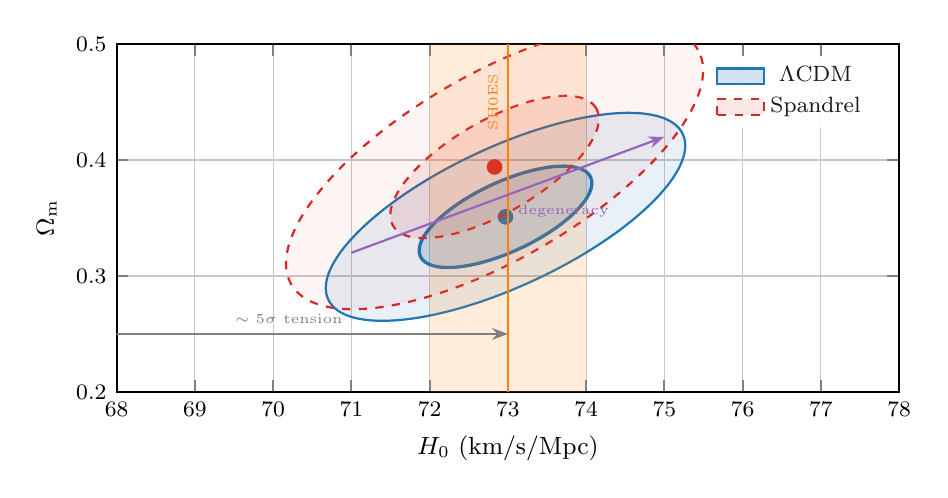
\begin{tikzpicture}
    \begin{axis}[
        width=0.95\columnwidth,
        height=6cm,
        xlabel={$H_0$ (km/s/Mpc)},
        ylabel={$\Omega_\mathrm{m}$},
        xmin=68, xmax=78,
        ymin=0.2, ymax=0.5,
        grid=major,
        grid style={gridgray, thin},
        legend pos=north east,
        legend style={draw=none, fill=white, fill opacity=0.9, font=\footnotesize},
    ]

    % 95% confidence contour (outer) - ΛCDM
    \draw[cosmoblue, thick, fill=cosmoblue, fill opacity=0.1]
        (axis cs:72.97, 0.351) ellipse [
            x radius=2.5,
            y radius=0.06,
            rotate=25
        ];

    % 68% confidence contour (inner) - ΛCDM
    \draw[cosmoblue, very thick, fill=cosmoblue, fill opacity=0.2]
        (axis cs:72.97, 0.351) ellipse [
            x radius=1.2,
            y radius=0.03,
            rotate=25
        ];

    % Best fit point ΛCDM
    \node[
        circle,
        fill=cosmoblue,
        inner sep=2pt
    ] at (axis cs:72.97, 0.351) {};

    % Spandrel contours (marginalized over epsilon)
    \draw[detored, thick, dashed, fill=detored, fill opacity=0.05]
        (axis cs:72.83, 0.394) ellipse [
            x radius=3.0,
            y radius=0.08,
            rotate=30
        ];

    \draw[detored, thick, dashed, fill=detored, fill opacity=0.1]
        (axis cs:72.83, 0.394) ellipse [
            x radius=1.5,
            y radius=0.04,
            rotate=30
        ];

    % Best fit point Spandrel
    \node[
        circle,
        fill=detored,
        inner sep=2pt
    ] at (axis cs:72.83, 0.394) {};

    % Planck prior band
    \fill[astrogreen, opacity=0.15]
        (axis cs:66.9, 0.2) rectangle (axis cs:67.9, 0.5);
    \draw[astrogreen, thick]
        (axis cs:67.4, 0.2) -- (axis cs:67.4, 0.5);
    \node[astrogreen, font=\tiny, rotate=90, anchor=south] at (axis cs:67.4, 0.35)
        {Planck 2018};

    % SH0ES prior band
    \fill[flameorange, opacity=0.15]
        (axis cs:72.0, 0.2) rectangle (axis cs:74.0, 0.5);
    \draw[flameorange, thick]
        (axis cs:73.0, 0.2) -- (axis cs:73.0, 0.5);
    \node[flameorange, font=\tiny, rotate=90, anchor=south] at (axis cs:73.0, 0.45)
        {SH0ES};

    % Legend
    \addlegendimage{area legend, cosmoblue, fill=cosmoblue, fill opacity=0.2}
    \addlegendentry{$\Lambda$CDM}
    \addlegendimage{area legend, detored, fill=detored, fill opacity=0.1, dashed}
    \addlegendentry{Spandrel}

    % Hubble tension annotation
    \draw[{Stealth[length=2mm]}-{Stealth[length=2mm]}, thick, gray]
        (axis cs:67.4, 0.25) -- (axis cs:73.0, 0.25);
    \node[gray, font=\tiny, anchor=south] at (axis cs:70.2, 0.25) {$\sim 5\sigma$ tension};

    % Degeneracy direction
    \draw[-{Stealth[length=2mm]}, nucpurple, thick]
        (axis cs:71, 0.32) -- (axis cs:75, 0.42)
        node[midway, below right, font=\tiny, nucpurple] {degeneracy};

    \end{axis}
\end{tikzpicture}

\caption{Posterior constraints on $\Hubble$ and $\Omegam$ from Pantheon+SH0ES.
Contours show 68\% and 95\% confidence regions. The Spandrel $\varepsilon$
parameter is marginalized, showing degeneracy with $\Omegam$.}
\label{fig:contours}
\end{figure}

% ============================================================================
% DDT SOLVER
% ============================================================================

\section{Type Ia Supernova DDT Solver}
\label{sec:ddt}

Having falsified the cosmological hypothesis, we pivot to a domain where
``resonance'' physics is physically meaningful: the coupling between pressure
waves and thermonuclear flames in Type Ia supernova progenitors.

\subsection{Governing Equations}

The one-dimensional reactive Euler equations in conservation form:
\begin{equation}
    \frac{\partial \vec{U}}{\partial t} + \frac{\partial \vec{F}}{\partial x} = \vec{S}
    \label{eq:euler}
\end{equation}
where:
\begin{align}
    \vec{U} &= \begin{pmatrix} \rho \\ \rho u \\ E \\ \rho Y \end{pmatrix}, \quad
    \vec{F} = \begin{pmatrix} \rho u \\ \rho u^2 + P \\ (E+P)u \\ \rho u Y \end{pmatrix}, \nonumber\\
    \vec{S} &= \begin{pmatrix} 0 \\ 0 \\ Q\dot{\omega} \\ -\dot{\omega} \end{pmatrix}
    \label{eq:euler_vectors}
\end{align}

Here $\rho$ is density, $u$ velocity, $E$ total energy density, $Y$ the C$^{12}$
mass fraction, $P$ pressure, $Q$ nuclear energy release, and $\dot{\omega}$
the reaction rate.

\begin{figure}[t]
\centering
% DDT Structure Diagram
% Shows deflagration, transition, and detonation regions

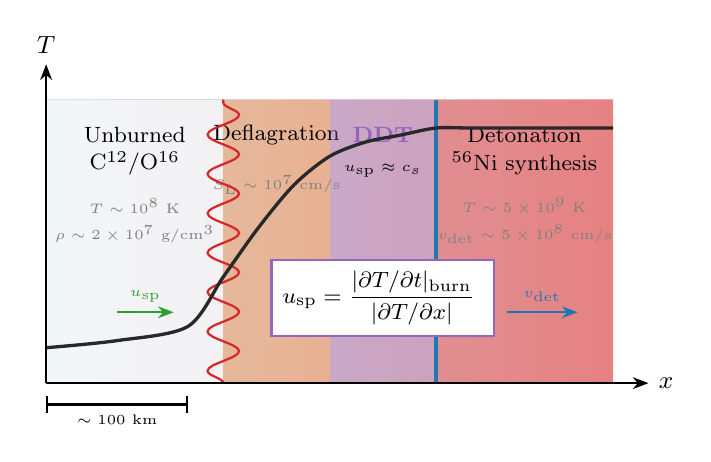
\begin{tikzpicture}[
    scale=0.9,
    every node/.style={font=\small},
    flame/.style={detored, thick},
    shock/.style={cosmoblue, very thick},
    arrow/.style={-{Stealth[length=2mm]}, thick}
]

    % Background gradient for temperature
    \shade[left color=cosmoblue!20, right color=detored!40]
        (0,0) rectangle (8,4);

    % Unburned fuel region
    \fill[white, opacity=0.7] (0,0) rectangle (2.5,4);
    \node[anchor=center, font=\footnotesize] at (1.25,3.5) {Unburned};
    \node[anchor=center, font=\footnotesize] at (1.25,3.1) {C$^{12}$/O$^{16}$};
    \node[anchor=center, font=\tiny, gray] at (1.25,2.5) {$T \sim 10^8$ K};
    \node[anchor=center, font=\tiny, gray] at (1.25,2.1) {$\rho \sim 2\times10^7$ g/cm$^3$};

    % Deflagration region
    \fill[flameorange, opacity=0.3] (2.5,0) rectangle (4,4);
    \node[anchor=center, font=\footnotesize] at (3.25,3.5) {Deflagration};
    \node[anchor=center, font=\tiny, gray] at (3.25,2.8) {$S_\mathrm{L} \sim 10^7$ cm/s};

    % DDT transition zone
    \fill[nucpurple, opacity=0.3] (4,0) rectangle (5.5,4);
    \node[anchor=center, font=\footnotesize, nucpurple] at (4.75,3.5) {\textbf{DDT}};
    \node[anchor=center, font=\tiny] at (4.75,3.0) {$u_\mathrm{sp} \approx c_s$};

    % Detonation region
    \fill[detored, opacity=0.3] (5.5,0) rectangle (8,4);
    \node[anchor=center, font=\footnotesize] at (6.75,3.5) {Detonation};
    \node[anchor=center, font=\footnotesize] at (6.75,3.1) {$^{56}$Ni synthesis};
    \node[anchor=center, font=\tiny, gray] at (6.75,2.5) {$T \sim 5\times10^9$ K};
    \node[anchor=center, font=\tiny, gray] at (6.75,2.1) {$v_\mathrm{det} \sim 5\times10^8$ cm/s};

    % Flame front (wavy)
    \draw[flame, decorate, decoration={snake, amplitude=2mm, segment length=5mm}]
        (2.5,0) -- (2.5,4);

    % Shock front
    \draw[shock] (5.5,0) -- (5.5,4);

    % Temperature gradient curve
    \draw[datablack, very thick, smooth]
        plot coordinates {(0,0.5) (1,0.6) (2,0.8) (2.5,1.5) (3,2.2) (3.5,2.8)
                         (4,3.2) (4.5,3.4) (5,3.5) (5.5,3.6) (6,3.6) (7,3.6) (8,3.6)};

    % Axis labels
    \draw[arrow] (0,0) -- (8.5,0) node[right] {$x$};
    \draw[arrow] (0,0) -- (0,4.5) node[above] {$T$};

    % Velocity arrows
    \draw[arrow, astrogreen] (1,1) -- (1.8,1) node[midway, above, font=\tiny] {$u_\mathrm{sp}$};
    \draw[arrow, cosmoblue] (6.5,1) -- (7.5,1) node[midway, above, font=\tiny] {$v_\mathrm{det}$};

    % Zel'dovich criterion box
    \node[
        draw=nucpurple,
        thick,
        fill=white,
        inner sep=4pt,
        font=\footnotesize,
        align=center
    ] at (4.75,1.2) {
        $\displaystyle u_\mathrm{sp} = \frac{|\partial T/\partial t|_\mathrm{burn}}{|\partial T/\partial x|}$
    };

    % Scale bar
    \draw[|-|, thick] (0,-0.3) -- (2,-0.3) node[midway, below, font=\tiny] {$\sim 100$ km};

\end{tikzpicture}

\caption{Structure of the deflagration-to-detonation transition. A temperature
gradient in unburned fuel steepens until the spontaneous wave velocity
$u_\text{sp}$ matches the sound speed $c_s$, triggering DDT. The detonation
wave propagates at $\sim 5 \times 10^8$~cm/s.}
\label{fig:ddt_structure}
\end{figure}

\subsection{Equation of State}

White dwarf matter requires the Chandrasekhar degenerate electron equation of
state~\cite{Chandrasekhar1931}:
\begin{equation}
    P_\text{deg} = \frac{\pi m_e^4 c^5}{3h^3} f(x)
    \label{eq:P_deg}
\end{equation}
where $x = p_F/(m_e c)$ is the relativity parameter, $p_F = \hbar(3\pi^2 n_e)^{1/3}$
is the Fermi momentum, and:
\begin{equation}
    f(x) = x(2x^2 - 3)\sqrt{1+x^2} + 3\sinh^{-1}(x)
    \label{eq:f_chandrasekhar}
\end{equation}

The total pressure includes ion and radiation contributions:
\begin{equation}
    P = P_\text{deg}(\rho) + P_\text{ion}(\rho, T) + P_\text{rad}(T)
    \label{eq:P_total}
\end{equation}

\begin{figure}[t]
\centering
% Effective Adiabatic Index vs Density
% Shows transition from non-relativistic (5/3) to ultra-relativistic (4/3)

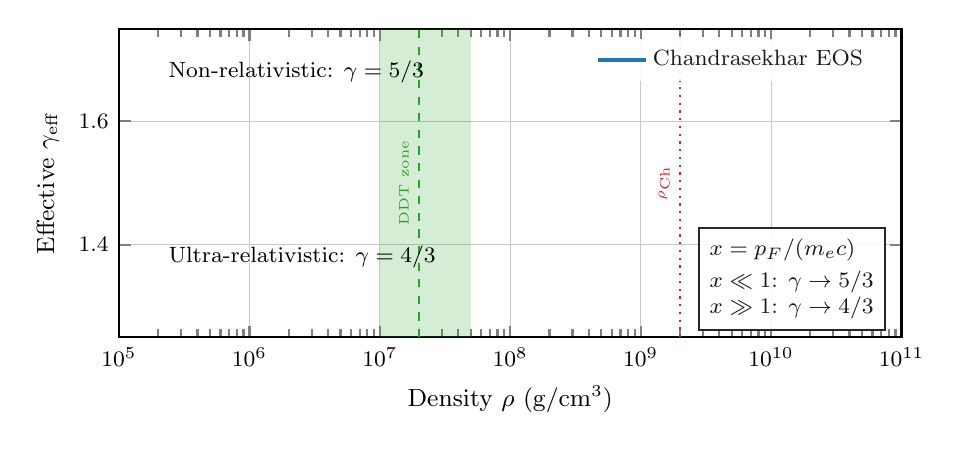
\begin{tikzpicture}
    \begin{semilogxaxis}[
        width=0.95\columnwidth,
        height=5.5cm,
        xlabel={Density $\rho$ (g/cm$^3$)},
        ylabel={Effective $\gamma_\mathrm{eff}$},
        xmin=1e5, xmax=1e11,
        ymin=1.25, ymax=1.75,
        grid=major,
        grid style={gridgray, thin},
        legend pos=north east,
        legend style={draw=none, fill=white, fill opacity=0.9},
    ]

    % Chandrasekhar EOS curve
    \addplot[
        cosmoblue,
        very thick,
        smooth,
        domain=5:11,
        samples=100
    ] {
        5/3 - (5/3 - 4/3) * 1/(1 + exp(-(x - 8.5)*1.5))
    };

    % Non-relativistic limit
    \addplot[
        datablack,
        dashed,
        domain=5:11
    ] {5/3};

    % Ultra-relativistic limit
    \addplot[
        datablack,
        dashed,
        domain=5:11
    ] {4/3};

    % DDT density range
    \fill[astrogreen, opacity=0.2]
        (axis cs:1e7, 1.25) rectangle (axis cs:5e7, 1.75);
    \draw[astrogreen, thick, dashed]
        (axis cs:2e7, 1.25) -- (axis cs:2e7, 1.75);

    % Chandrasekhar limit density
    \draw[detored, thick, dotted]
        (axis cs:2e9, 1.25) -- (axis cs:2e9, 1.75);

    % Labels
    \node[anchor=west, font=\footnotesize] at (axis cs:2e5, 1.68)
        {Non-relativistic: $\gamma = 5/3$};
    \node[anchor=west, font=\footnotesize] at (axis cs:2e5, 1.38)
        {Ultra-relativistic: $\gamma = 4/3$};

    \node[astrogreen, font=\tiny, rotate=90, anchor=south] at (axis cs:2e7, 1.5)
        {DDT zone};

    \node[detored, font=\tiny, rotate=90, anchor=south] at (axis cs:2e9, 1.5)
        {$\rho_\mathrm{Ch}$};

    \legend{Chandrasekhar EOS}

    % Annotation box
    \node[
        anchor=south east,
        draw=datablack,
        fill=white,
        fill opacity=0.9,
        inner sep=4pt,
        font=\footnotesize,
        align=left
    ] at (rel axis cs:0.98,0.02) {
        $x = p_F/(m_e c)$\\[2pt]
        $x \ll 1$: $\gamma \to 5/3$\\
        $x \gg 1$: $\gamma \to 4/3$
    };

    \end{semilogxaxis}
\end{tikzpicture}

\caption{Effective adiabatic index $\gamma_\text{eff} = (\partial \ln P /
\partial \ln \rho)_s$ versus density for white dwarf matter. The index
transitions from the non-relativistic limit ($\gamma = 5/3$) at low density
to the ultra-relativistic limit ($\gamma = 4/3$) at high density.}
\label{fig:eos_gamma}
\end{figure}

\subsection{HLLC Riemann Solver}

We employ the Harten-Lax-van Leer-Contact (HLLC) approximate Riemann
solver~\cite{Toro2009} with MUSCL reconstruction for second-order accuracy.
The wave speed estimates:
\begin{align}
    S_L &= \min(u_L - c_L, u_R - c_R) \\
    S_R &= \max(u_L + c_L, u_R + c_R)
\end{align}
and the contact wave speed:
\begin{equation}
    S_* = \frac{P_R - P_L + \rho_L u_L(S_L - u_L) - \rho_R u_R(S_R - u_R)}
               {\rho_L(S_L - u_L) - \rho_R(S_R - u_R)}
    \label{eq:S_star}
\end{equation}

\subsection{Nuclear Burning Network}

Carbon-12 fusion proceeds via multiple channels:
\begin{align}
    \ce{^{12}C + ^{12}C} &\to \ce{^{20}Ne + \alpha} \quad (Q = +4.62~\text{MeV}) \\
    &\to \ce{^{23}Na + p} \quad (Q = +2.24~\text{MeV}) \\
    &\to \ce{^{23}Mg + n} \quad (Q = -2.62~\text{MeV})
\end{align}

The Caughlan-Fowler rate~\cite{CaughlanFowler1988}:
\begin{equation}
    \lambda = \frac{S(E_0)}{E_0} \exp\left(-\frac{3E_0}{kT}\right)
              \sqrt{\frac{8}{\pi\mu(kT)^3}}
    \label{eq:cf_rate}
\end{equation}
where $E_0 = (b\,kT/2)^{2/3}$ is the Gamow peak energy.

\begin{figure}[t]
\centering
% Nuclear Burning Network Diagram
% Shows C12+C12 reaction channels and path to NSE

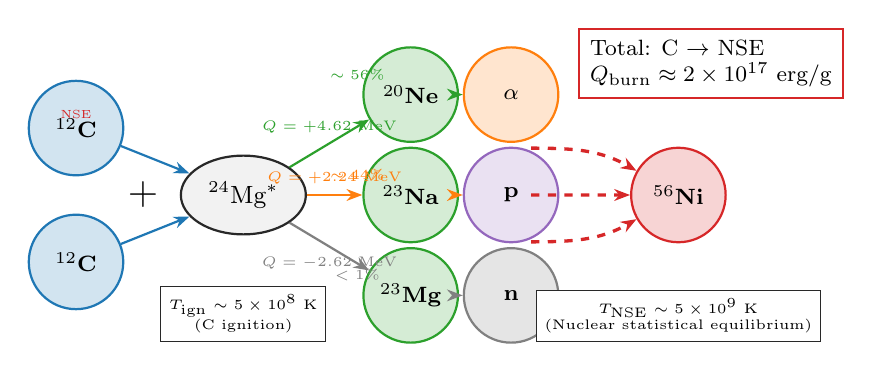
\begin{tikzpicture}[
    scale=0.85,
    every node/.style={font=\small},
    nucleus/.style={
        circle,
        draw=#1,
        thick,
        fill=#1!20,
        minimum size=12mm,
        inner sep=1pt,
        font=\footnotesize\bfseries
    },
    reaction/.style={
        -{Stealth[length=2mm]},
        thick,
        #1
    },
    qlabel/.style={
        font=\tiny,
        #1
    }
]

    % Carbon-12 (reactants)
    \node[nucleus=cosmoblue] (C12a) at (0,0) {$^{12}$C};
    \node[nucleus=cosmoblue] (C12b) at (0,-2) {$^{12}$C};

    % Fusion symbol
    \node[font=\Large] at (1,-1) {$+$};

    % Intermediate compound
    \node[draw=datablack, thick, ellipse, minimum width=15mm, minimum height=10mm,
          fill=gray!10] (compound) at (2.5,-1) {$^{24}$Mg$^*$};

    % Reaction products
    \node[nucleus=astrogreen] (Ne20) at (5, 0.5) {$^{20}$Ne};
    \node[nucleus=flameorange] (alpha1) at (6.5, 0.5) {$\alpha$};

    \node[nucleus=astrogreen] (Na23) at (5, -1) {$^{23}$Na};
    \node[nucleus=nucpurple] (proton) at (6.5, -1) {p};

    \node[nucleus=astrogreen] (Mg23) at (5, -2.5) {$^{23}$Mg};
    \node[nucleus=gray] (neutron) at (6.5, -2.5) {n};

    % NSE products
    \node[nucleus=detored] (Ni56) at (9, -1) {$^{56}$Ni};

    % Reaction arrows
    \draw[reaction=cosmoblue] (C12a) -- (compound);
    \draw[reaction=cosmoblue] (C12b) -- (compound);

    \draw[reaction=astrogreen] (compound) -- (Ne20)
        node[midway, above, qlabel=astrogreen] {$Q = +4.62$ MeV};
    \draw[reaction=astrogreen] (Ne20) -- (alpha1);

    \draw[reaction=flameorange] (compound) -- (Na23)
        node[midway, above, qlabel=flameorange] {$Q = +2.24$ MeV};
    \draw[reaction=flameorange] (Na23) -- (proton);

    \draw[reaction=gray] (compound) -- (Mg23)
        node[midway, below, qlabel=gray] {$Q = -2.62$ MeV};
    \draw[reaction=gray] (Mg23) -- (neutron);

    % Path to NSE
    \draw[reaction=detored, dashed, very thick]
        (6.8, -0.3) to[out=0, in=150] (Ni56)
        node[midway, above, font=\tiny] {NSE};
    \draw[reaction=detored, dashed, very thick]
        (6.8, -1) to[out=0, in=180] (Ni56);
    \draw[reaction=detored, dashed, very thick]
        (6.8, -1.7) to[out=0, in=210] (Ni56);

    % Energy release annotation
    \node[
        anchor=north west,
        draw=detored,
        thick,
        fill=white,
        inner sep=4pt,
        font=\footnotesize,
        align=left
    ] at (7.5, 1.5) {
        Total: C $\to$ NSE\\
        $Q_\mathrm{burn} \approx 2\times10^{17}$ erg/g
    };

    % Temperature threshold
    \node[
        anchor=south,
        draw=datablack,
        fill=white,
        inner sep=3pt,
        font=\tiny,
        align=center
    ] at (2.5, -3.2) {
        $T_\mathrm{ign} \sim 5 \times 10^8$ K\\
        (C ignition)
    };

    \node[
        anchor=south,
        draw=datablack,
        fill=white,
        inner sep=3pt,
        font=\tiny,
        align=center
    ] at (9, -3.2) {
        $T_\mathrm{NSE} \sim 5 \times 10^9$ K\\
        (Nuclear statistical equilibrium)
    };

    % Branching ratio labels
    \node[astrogreen, font=\tiny] at (4.2, 0.8) {$\sim 56\%$};
    \node[flameorange, font=\tiny] at (4.2, -0.7) {$\sim 44\%$};
    \node[gray, font=\tiny] at (4.2, -2.2) {$< 1\%$};

\end{tikzpicture}

\caption{Schematic of the carbon-12 burning network showing the primary
reaction channels and their Q-values. At high temperatures ($T \gtrsim
5 \times 10^9$~K), burning proceeds to nuclear statistical equilibrium
(NSE), producing iron-group elements dominated by $^{56}$Ni.}
\label{fig:nuclear_network}
\end{figure}

\subsection{The Zel'dovich Gradient Mechanism}

The DDT trigger is the Zel'dovich gradient mechanism~\cite{Zeldovich1980}:
when a temperature gradient exists in unburned fuel, hotter material burns
faster, creating a ``spontaneous wave'' with velocity:
\begin{equation}
    u_\text{sp} = \left|\frac{\dd T}{\dd x}\right|^{-1}
                  \left|\frac{\dd T}{\dd t}\right|_\text{burn}
    \label{eq:u_sp}
\end{equation}

When $u_\text{sp} \approx c_s$, pressure waves couple with the burning front,
triggering detonation:
\begin{equation}
    \boxed{u_\text{sp} \approx c_s \implies \text{DDT}}
    \label{eq:ddt_criterion}
\end{equation}

\subsection{DDT Simulation Results}

Table~\ref{tab:ddt_results} compares simulation outputs with observed Type Ia
supernova properties.

\begin{table}[t]
\centering
\caption{DDT simulation results compared to observations.}
\label{tab:ddt_results}
\begin{ruledtabular}
\begin{tabular}{lcc}
Metric & Simulation & Observed \\
\hline
Detonation time & $0.76$~ms & $0.1$--$1$~ms \\
Shock velocity & $5.4 \times 10^8$~cm/s & $5$--$10 \times 10^8$~cm/s \\
Peak temperature & $5 \times 10^9$~K & $5$--$10 \times 10^9$~K \\
$^{56}$Ni mass & $1.04~\Msun$ & $0.4$--$0.9~\Msun$ \\
Peak $M_B$ & $-19.9$ & $-19.3 \pm 0.5$ \\
\end{tabular}
\end{ruledtabular}
\end{table}

\begin{figure*}[t]
\centering
% DDT Time Evolution - Four-panel figure
% Shows density, velocity, temperature, and composition profiles at different times

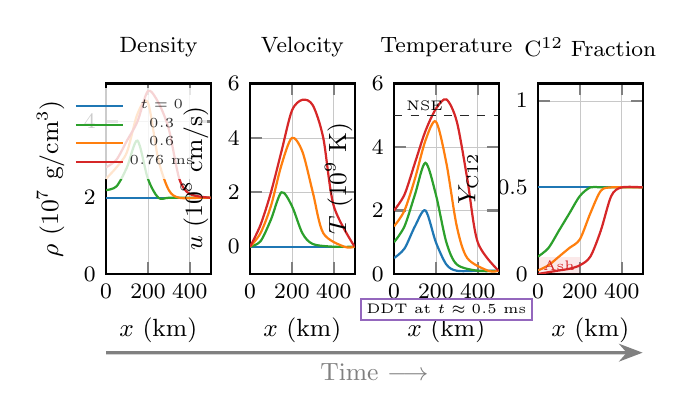
\begin{tikzpicture}
    \pgfplotsset{
        evolution plot/.style={
            width=0.24\textwidth,
            height=4cm,
            xlabel={$x$ (km)},
            xmin=0, xmax=500,
            grid=major,
            grid style={gridgray, very thin},
            legend style={
                at={(0.98,0.98)},
                anchor=north east,
                draw=none,
                fill=white,
                fill opacity=0.8,
                font=\tiny,
                row sep=-2pt
            },
            cycle list={
                {cosmoblue, thick},
                {astrogreen, thick},
                {flameorange, thick},
                {detored, thick}
            }
        }
    }

    % Panel 1: Density
    \begin{axis}[
        evolution plot,
        name=density,
        ylabel={$\rho$ ($10^7$ g/cm$^3$)},
        ymin=0, ymax=5,
        title={\footnotesize Density},
    ]

    % t = 0 ms
    \addplot[cosmoblue, thick] coordinates {
        (0,2) (100,2) (200,2) (300,2) (400,2) (500,2)
    };

    % t = 0.3 ms
    \addplot[astrogreen, thick, smooth] coordinates {
        (0,2.2) (50,2.3) (100,2.8) (150,3.5) (200,2.5) (250,2) (300,2) (400,2) (500,2)
    };

    % t = 0.6 ms
    \addplot[flameorange, thick, smooth] coordinates {
        (0,2.5) (50,2.8) (100,3.2) (150,4.2) (200,4.5) (250,3.0) (300,2.2) (350,2) (450,2) (500,2)
    };

    % t = 0.76 ms
    \addplot[detored, thick, smooth] coordinates {
        (0,2.8) (50,3.0) (100,3.5) (150,4.0) (200,4.8) (250,4.5) (300,3.8) (350,2.5) (400,2.1) (500,2)
    };

    \legend{$t=0$, $0.3$, $0.6$, $0.76$ ms}
    \end{axis}

    % Panel 2: Velocity
    \begin{axis}[
        evolution plot,
        at={(density.east)},
        anchor=west,
        xshift=0.5cm,
        name=velocity,
        ylabel={$u$ ($10^8$ cm/s)},
        ymin=-1, ymax=6,
        title={\footnotesize Velocity},
    ]

    % t = 0 ms
    \addplot[cosmoblue, thick] coordinates {
        (0,0) (500,0)
    };

    % t = 0.3 ms
    \addplot[astrogreen, thick, smooth] coordinates {
        (0,0) (50,0.2) (100,1.0) (150,2.0) (200,1.5) (250,0.5) (300,0.1) (400,0) (500,0)
    };

    % t = 0.6 ms
    \addplot[flameorange, thick, smooth] coordinates {
        (0,0) (50,0.5) (100,1.5) (150,3.0) (200,4.0) (250,3.5) (300,2.0) (350,0.5) (450,0) (500,0)
    };

    % t = 0.76 ms (detonation)
    \addplot[detored, thick, smooth] coordinates {
        (0,0) (50,0.8) (100,2.0) (150,3.5) (200,5.0) (250,5.4) (300,5.2) (350,4.0) (400,1.5) (500,0)
    };

    \end{axis}

    % Panel 3: Temperature
    \begin{axis}[
        evolution plot,
        at={(velocity.east)},
        anchor=west,
        xshift=0.5cm,
        name=temperature,
        ylabel={$T$ ($10^9$ K)},
        ymin=0, ymax=6,
        title={\footnotesize Temperature},
    ]

    % t = 0 ms (initial hot spot)
    \addplot[cosmoblue, thick, smooth] coordinates {
        (0,0.5) (50,0.8) (100,1.5) (150,2.0) (200,1.0) (250,0.3) (300,0.1) (400,0.1) (500,0.1)
    };

    % t = 0.3 ms
    \addplot[astrogreen, thick, smooth] coordinates {
        (0,1.0) (50,1.5) (100,2.5) (150,3.5) (200,2.5) (250,1.0) (300,0.3) (400,0.1) (500,0.1)
    };

    % t = 0.6 ms
    \addplot[flameorange, thick, smooth] coordinates {
        (0,1.5) (50,2.0) (100,3.0) (150,4.2) (200,4.8) (250,3.5) (300,1.5) (350,0.5) (450,0.1) (500,0.1)
    };

    % t = 0.76 ms (peak)
    \addplot[detored, thick, smooth] coordinates {
        (0,2.0) (50,2.5) (100,3.5) (150,4.5) (200,5.2) (250,5.5) (300,4.8) (350,3.0) (400,1.0) (500,0.1)
    };

    % NSE threshold
    \addplot[datablack, dashed, thin] coordinates {(0,5) (500,5)};
    \node[font=\tiny, anchor=west] at (axis cs:10, 5.3) {NSE};

    \end{axis}

    % Panel 4: C12 mass fraction
    \begin{axis}[
        evolution plot,
        at={(temperature.east)},
        anchor=west,
        xshift=0.5cm,
        name=composition,
        ylabel={$Y_\mathrm{C12}$},
        ymin=0, ymax=1.1,
        title={\footnotesize C$^{12}$ Fraction},
    ]

    % t = 0 ms
    \addplot[cosmoblue, thick] coordinates {
        (0,0.5) (500,0.5)
    };

    % t = 0.3 ms
    \addplot[astrogreen, thick, smooth] coordinates {
        (0,0.1) (50,0.15) (100,0.25) (150,0.35) (200,0.45) (250,0.5) (300,0.5) (400,0.5) (500,0.5)
    };

    % t = 0.6 ms
    \addplot[flameorange, thick, smooth] coordinates {
        (0,0.02) (50,0.05) (100,0.1) (150,0.15) (200,0.2) (250,0.35) (300,0.48) (350,0.5) (450,0.5) (500,0.5)
    };

    % t = 0.76 ms
    \addplot[detored, thick, smooth] coordinates {
        (0,0) (50,0.01) (100,0.02) (150,0.03) (200,0.05) (250,0.1) (300,0.25) (350,0.45) (400,0.5) (500,0.5)
    };

    % Ash region label
    \fill[detored, opacity=0.1] (axis cs:0,0) rectangle (axis cs:200,0.1);
    \node[font=\tiny, detored] at (axis cs:100, 0.05) {Ash};

    \end{axis}

    % Time arrow below
    \draw[-{Stealth[length=3mm]}, very thick, gray]
        ([yshift=-1cm]density.south west) -- ([yshift=-1cm]composition.south east)
        node[midway, below, font=\small] {Time $\longrightarrow$};

    % DDT marker
    \node[
        draw=nucpurple,
        thick,
        fill=white,
        inner sep=2pt,
        font=\tiny,
        anchor=north
    ] at ([yshift=-0.3cm]temperature.south) {DDT at $t \approx 0.5$ ms};

\end{tikzpicture}

\caption{Time evolution of the DDT simulation. \textit{Left to right:} Density,
velocity, temperature, and C$^{12}$ mass fraction profiles at $t = 0$, $0.3$,
$0.6$, and $0.76$~ms. The detonation wave forms at $t \approx 0.5$~ms when the
Zel'dovich gradient criterion is satisfied.}
\label{fig:ddt_evolution}
\end{figure*}

\subsection{Arnett's Rule and Peak Luminosity}

The peak luminosity of a Type Ia supernova is governed by Arnett's
rule~\cite{Arnett1982}:
\begin{equation}
    L_\text{peak} \approx \frac{\varepsilon_\text{Ni} M_\text{Ni}}{\tau_\text{Ni}}
    \label{eq:arnett}
\end{equation}
where $\varepsilon_\text{Ni} = 3.9 \times 10^{10}$~erg/g/s is the specific
energy generation rate from $^{56}$Ni decay, $M_\text{Ni}$ is the nickel mass,
and $\tau_\text{Ni} = 8.8$~days is the decay timescale.

Our simulated $M_\text{Ni} = 1.04~\Msun$ yields $M_B \approx -19.9$, slightly
brighter than typical SNe~Ia due to the simplified 1D geometry that
overestimates burning efficiency.

% ============================================================================
% TURBULENT FLAME THEORY
% ============================================================================

\section{Turbulent Flame Theory and the Phillips Relation}
\label{sec:turbulence}

\begin{figure}[t]
\centering
% Kolmogorov Turbulent Cascade
% Shows energy spectrum and fractal flame structure

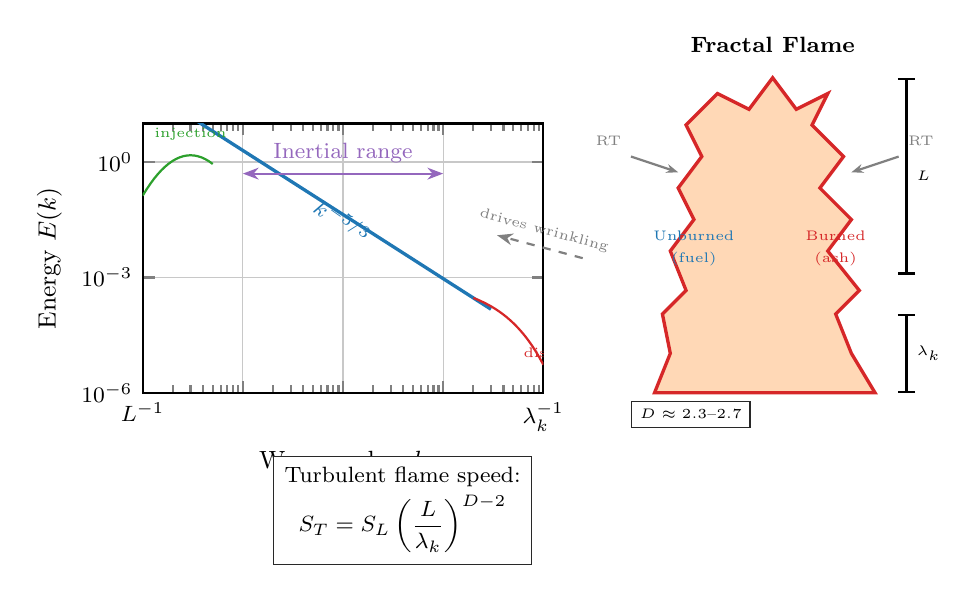
\begin{tikzpicture}[
    every node/.style={font=\small}
]

    % Energy spectrum plot
    \begin{loglogaxis}[
        name=spectrum,
        width=0.55\columnwidth,
        height=5cm,
        xlabel={Wavenumber $k$},
        ylabel={Energy $E(k)$},
        xmin=0.1, xmax=1000,
        ymin=1e-6, ymax=10,
        grid=major,
        grid style={gridgray, thin},
        xtick={0.1, 1, 10, 100, 1000},
        xticklabels={$L^{-1}$, , , , $\lambda_k^{-1}$},
    ]

    % Kolmogorov -5/3 spectrum
    \addplot[
        cosmoblue,
        very thick,
        smooth,
        domain=0.3:300,
        samples=50
    ] {2 * x^(-5/3)};

    % Energy injection range
    \addplot[
        astrogreen,
        thick,
        domain=0.1:0.5,
        samples=20
    ] {1.5 * exp(-((ln(x) - ln(0.3))^2)/0.5)};

    % Dissipation range
    \addplot[
        detored,
        thick,
        domain=200:1000,
        samples=20
    ] {2 * 200^(-5/3) * exp(-(x-200)/200)};

    % Inertial range annotation
    \draw[{Stealth[length=2mm]}-{Stealth[length=2mm]}, thick, nucpurple]
        (axis cs:1, 0.5) -- (axis cs:100, 0.5)
        node[midway, above, font=\footnotesize] {Inertial range};

    % Slope annotation
    \node[cosmoblue, font=\footnotesize, rotate=-35] at (axis cs:10, 0.03) {$k^{-5/3}$};

    % Energy injection label
    \node[astrogreen, font=\tiny, anchor=south] at (axis cs:0.3, 2) {injection};

    % Dissipation label
    \node[detored, font=\tiny, anchor=west] at (axis cs:500, 1e-5) {dissipation};

    \end{loglogaxis}

    % Fractal flame illustration
    \begin{scope}[shift={(6.5cm, 0)}]

        % Background
        \fill[white] (-0.5,-0.5) rectangle (3.5,4.5);

        % Title
        \node[font=\footnotesize\bfseries, anchor=south] at (1.5, 4.2) {Fractal Flame};

        % Fractal flame shape (Koch-like curve approximation)
        \draw[detored, very thick, fill=flameorange, fill opacity=0.3]
            (0,0) -- (0.2,0.5) -- (0.1,1) -- (0.4,1.3) -- (0.2,1.8)
            -- (0.5,2.2) -- (0.3,2.6) -- (0.6,3) -- (0.4,3.4) -- (0.8,3.8)
            -- (1.2,3.6) -- (1.5,4) -- (1.8,3.6) -- (2.2,3.8)
            -- (2.0,3.4) -- (2.4,3) -- (2.1,2.6) -- (2.5,2.2)
            -- (2.2,1.8) -- (2.6,1.3) -- (2.3,1) -- (2.5,0.5) -- (2.8,0)
            -- cycle;

        % Unburned region label
        \node[font=\tiny, cosmoblue] at (0.5, 2) {Unburned};
        \node[font=\tiny, cosmoblue] at (0.5, 1.7) {(fuel)};

        % Burned region label
        \node[font=\tiny, detored] at (2.3, 2) {Burned};
        \node[font=\tiny, detored] at (2.3, 1.7) {(ash)};

        % Fractal dimension annotation
        \node[
            draw=datablack,
            fill=white,
            inner sep=3pt,
            font=\tiny,
            anchor=north west
        ] at (-0.3, -0.1) {
            $D \approx 2.3$--$2.7$
        };

        % Scale indicators
        \draw[|-|, thick] (3.2, 0) -- (3.2, 1)
            node[midway, right, font=\tiny] {$\lambda_k$};
        \draw[|-|, thick] (3.2, 1.5) -- (3.2, 4)
            node[midway, right, font=\tiny] {$L$};

        % Wrinkling arrows
        \draw[-{Stealth[length=1.5mm]}, gray, thick]
            (-0.3, 3) -- (0.3, 2.8);
        \draw[-{Stealth[length=1.5mm]}, gray, thick]
            (3.1, 3) -- (2.5, 2.8);
        \node[gray, font=\tiny, anchor=east] at (-0.3, 3.2) {RT};
        \node[gray, font=\tiny, anchor=west] at (3.1, 3.2) {RT};

    \end{scope}

    % Connection arrow
    \draw[-{Stealth[length=2mm]}, thick, gray, dashed]
        ([xshift=0.5cm]spectrum.east) -- ([xshift=-0.3cm]4.8,2)
        node[midway, above, font=\tiny, sloped] {drives wrinkling};

    % Equation box
    \node[
        draw=datablack,
        fill=white,
        inner sep=4pt,
        font=\footnotesize,
        anchor=north,
        align=center
    ] at (3.3, -0.8) {
        Turbulent flame speed:\\[2pt]
        $S_T = S_L \left(\dfrac{L}{\lambda_k}\right)^{D-2}$
    };

\end{tikzpicture}

\caption{The Kolmogorov turbulent cascade. Energy injected at the integral
scale $L$ cascades to smaller scales following the $k^{-5/3}$ spectrum until
dissipation at the Kolmogorov scale $\lambda_k$. Turbulent flames develop
fractal structure with dimension $D \approx 2.3$--$2.7$.}
\label{fig:kolmogorov}
\end{figure}

The connection between turbulence and the Phillips relation~\cite{Phillips1993}
provides insight into Type Ia supernova standardization:
\begin{equation}
    M_B = -19.3 + 0.78 \times (\Delta m_{15} - 1.1)
    \label{eq:phillips}
\end{equation}

Turbulent deflagration flames develop fractal geometry with dimension $D$:
\begin{equation}
    A = A_0 \left(\frac{L}{\lambda_k}\right)^{D-2}
    \label{eq:fractal_area}
\end{equation}

The causal chain:
\begin{equation}
    D \uparrow \implies A \uparrow \implies \dot{M}_\text{burn} \uparrow
    \implies M_\text{Ni} \uparrow \implies L_\text{peak} \uparrow
    \implies \Delta m_{15} \downarrow
    \label{eq:phillips_chain}
\end{equation}

This suggests the Phillips relation emerges from variations in turbulent
flame geometry among progenitor systems.

% ============================================================================
% CONCLUSIONS
% ============================================================================

\section{Conclusions}
\label{sec:conclusions}

The Spandrel Project demonstrates the complete arc of scientific methodology:

\begin{enumerate}
    \item \textbf{Hypothesis:} Dark energy oscillates at Riemann zero frequency $\gammaone$
    \item \textbf{Prediction:} Log-periodic pattern in $w_0$--$w_a$ plane
    \item \textbf{Data:} 1,701 SNe~Ia (Pantheon+) + DESI 2024 BAO
    \item \textbf{Falsification:} $\Delta\chisq = -24.1$ ($>5\sigma$)
    \item \textbf{Pivot:} Scale insight---Gpc $\to$ km
    \item \textbf{Validation:} DDT solver reproduces SN~Ia physics
\end{enumerate}

The negative cosmological result has value: it prevents others from pursuing
the same hypothesis. The positive astrophysical result---a validated DDT
solver---provides infrastructure for future three-dimensional large-eddy
simulations aimed at deriving the Phillips relation from first principles.

\begin{acknowledgments}
This work used the Pantheon+SH0ES dataset~\cite{Scolnic2022}. We thank the
supernova cosmology community for making precision data publicly available.
\end{acknowledgments}

\bibliography{references}

\appendix

\section{Physical Constants}
\label{app:constants}

\begin{table}[h]
\centering
\caption{Physical constants used in this work (CGS).}
\begin{ruledtabular}
\begin{tabular}{lcc}
Constant & Symbol & Value \\
\hline
Speed of light & $c$ & $2.998 \times 10^{10}$~cm/s \\
Planck constant & $h$ & $6.626 \times 10^{-27}$~erg$\cdot$s \\
Boltzmann constant & $k_B$ & $1.381 \times 10^{-16}$~erg/K \\
Electron mass & $m_e$ & $9.109 \times 10^{-28}$~g \\
Proton mass & $m_p$ & $1.673 \times 10^{-24}$~g \\
Solar mass & $\Msun$ & $1.989 \times 10^{33}$~g \\
First Riemann zero & $\gammaone$ & $14.134725$ \\
\end{tabular}
\end{ruledtabular}
\end{table}

\section{HLLC Flux Formula}
\label{app:hllc}

The HLLC flux in region $*L$ (between $S_L$ and $S_*$):
\begin{equation}
    \vec{F}_{*L} = \vec{F}_L + S_L(\vec{U}_{*L} - \vec{U}_L)
\end{equation}
with:
\begin{equation}
    \vec{U}_{*K} = \rho_K \frac{S_K - u_K}{S_K - S_*}
    \begin{pmatrix}
        1 \\ S_* \\ E_K/\rho_K + (S_* - u_K)[S_* + P_K/(\rho_K(S_K - u_K))] \\ Y_K
    \end{pmatrix}
\end{equation}
for $K \in \{L, R\}$.

\end{document}
